\documentclass[a4paper]{article}


\usepackage{alphabeta} 
\usepackage{enumitem} 
\usepackage{mathtools}
\usepackage{amsmath, amssymb} 
\usepackage{amsthm}
\usepackage{cancel} 
\usepackage[margin=0.70in]{geometry} 
\geometry{left=3cm,right=3cm,top=2.4cm,bottom=2.4cm}	%the page geometry as defined, A4=210x297mm
\usepackage{graphicx}
\usepackage{wrapfig}
\usepackage[center]{caption}
\usepackage{textcomp}
\usepackage{tabto}
\usepackage{layout}
\usepackage{bm}
\usepackage{minipage-marginpar}
\usepackage[dvipsnames]{xcolor}
\usepackage{hyperref}
\usepackage{dutchcal}
\usepackage{derivative}
\usepackage{esint}
%\usepackage{biblatex}
\usepackage{subcaption}
\usepackage{booktabs}\usepackage{derivative}
\usepackage[flushleft]{threeparttable}
\usepackage[capbesideposition=outside,capbesidesep=quad]{floatrow}
\usepackage{derivative}
\usepackage[thinc]{esdiff}
\usepackage{lipsum}
\usepackage{arydshln}
%%RENEW

\newtheorem{problem}{Άσκηση}
\newtheorem*{solution*}{Λύση}
\newtheorem{definition}{Ορισμός}[subsection]
\newtheorem{properties}{Ιδιότητες}[subsection]
\newtheorem{theorem}{Θεώρημα}[subsection]
\newtheorem{protash}{Πρόταση}[subsection]
\newtheorem{porisma}{Πόρισμα}[subsection]
\newtheorem{lemma}{Λήμμα}[subsection]
\newtheorem*{prooof}{Απόδειξη}
\newtheorem*{notes}{Παρατηρήσεις}
\newtheorem*{note}{Παρατήρηση}
\newtheorem*{app}{Εφαρμογή} 
\newtheorem*{example}{Παράδειγμα}
\newtheorem*{examples}{Παραδείγματα}


\newcommand\numberthis{\addtocounter{equation}{1}\tag{\theequation}}
%\renewcommand{\labelenumi}{\roman{enumi}}
\newcommand{\approxtext}[1]{\ensuremath{\stackrel{\text{#1}}{\approx}}}
\renewcommand{\figurename}{Εικόνα.}
\renewcommand{\tablename}{Πίνακας.}
%\renewcommand\refname{New References Header}
\renewcommand*\contentsname{Περιεχόμενα}
%\DeclareDerivative{\odv}{\mathrm{d}}


\begin{document}
\begin{titlepage}			%makes a title page. Remember to change the author, CID, username and group number to what is appropriate for you!
	\centering
	{\scshape\LARGE Εθνικό Μετσόβιο Πολυτεχνείο\par}
	{\scshape \LARGE Σ.Ε.Μ.Φ.Ε.\par}
	\vspace{1cm}
	{\huge\bfseries Νόμος Moseley με την μέθοδο των χαρακτηριστικών ακτίνων Χ από ραδιενεργούς πυρήνες\par}
	\vspace{1cm}
	{\Large\itshape Θωμόπουλος Σπύρος\par}		%remember to change these!
	
	%		{\large Group \@group\unskip\strut\par}
	{\large spyros.thomop@gmail.com/ ge19042@mail.ntua.gr\par \hfill \\}% 		%remember to change these!
	\vspace{1cm}
	{\large Ημερμονηνία Παράδοσης 17/05/2022\par}
\end{titlepage}

\subsection*{Σκοπός}
	Ο σκοπός της εν λόγω εργαστηριακής άσκησης είναι η καταγραφή της ενέργειας χαρακτηριστικών ακτίνων Χ που εκπέμπονται από ραδιενεργούς πυρήνες και κατ' επέκταση η επιβεβαίωση του νόμου Moseley.


\subsection*{Θεωρητικά Στοιχεία}
	
	Σε ένα άτομο η κατανομή των ηλεκτρονίων σε στοιβάδες και υποστοιβάδες καθορισμένης ενέργειας διέπεται από συγκεκριμένους κανόνες (Αρχή Ελάχιστης Ενέργειας, Απαγορευτική Αρχή Pauli, κανόνες Hund κλπ). Προκειμένου να απομακρύνουμε ένα ηλεκτρόνιο από το δυναμικό του πυρήνα θα πρέπει να του δώσουμε ένα κατάλληλο ποσό ενέργειας, μεγαλύτερο ή ίσο από την ενέργεια που απαιτείται για την συγκράτηση του ηλεκτρονίου στον πυρήνα,την λεγόμενη \textit{ενέργεια ιονισμού}. Αν το ηλεκτρόνιο βρίσκεται σε εσωτερικό φλοιό, τότε δημιουργείται μία οπή και το άτομο μεταβαίνει σε μία διεγερμένη κατάσταση. Η εν λόγω κατάσταση είναι σχεδόν στιγμιαία εφόσον το άτομο θα πρέπει να μεταβεί σε μία ενεργειακά χαμηλότερη, άρα ευσταθή.
	
	%Κατά την εν λόγω διαδικασία εκπέμπεται μία χαρακτηριστική Ηλεκτρομαγνητική ακτινοβολία συγκεκριμένου μήκους κύματος και το άτομο μεταβαίνει σε μία ενεργειακά υψηλότερη κατάσταση, στην οποία δεν δύναται να παραμείνει για μεγάλο χρονικό διάστημα και γι' αυτό πραγματοποιείται μία μετάβαση ενός ηλεκτρονίου υψηλότερης ενέργειας στην θέση εκείνου που έχει απομακρυνθεί από το άτομο. Αυτά ισχύουν για ηλεκρόνια του εξωτερικού φλοιού.
	
	%Για ηλεκτρόνια σε εσωτερικό φλοιό τα πράγματα είναι λίγο διαφορετικά. Πάλι, όταν προσλαμβάνουν ενέργεια μπορούν να ιονιστουν, να αποδράσουν δηλαδή από το δυναμικό του πυρήνα εκπέμποντας ταυτόχρονα ακτίνες Χ. Ενδέχεται επίσης να μην έχουμε εχπομπή Η/Μ ακτινοβολίας, αλλά απόδοση της ενέργειας του ηλεκτρονίου σε άλλα, ενεργειακά υψηλότερα ηλεκτρόνια το οποία διαφεύγουν (ηλεκτρόνια Auger).
	
	Η μετάβαση σε ενεργειακά χαμηλότερη κατάσταση πραγματοποιείται με την μετάπτωση κάποιου εξωτερικού ηλεκτρονίου στην οπή, δηλαδή στην ''θέση'' απ' όπου έχει απομακρυνθεί το εσωτερικό ηλεκτρόνιο. Τα αποτελέσματα αυτής της μετάπτωσης, που επιβάλλονται από την Αρχή Διατήρησης της Ενέργειας, καθώς ένα ηλεκτρόνιο χάνει ενέργεια, είναι δύο. Αρχικά, ενδέχεται να εκπεμφθεί Η/Μ ακτινοβολία Χ με ενέργεια ίση με την ενέργειακή διαφορά των δύο σταθμών μεταξύ των οποίων πραγματοποιείται η μετάβαση. Ακόμη, η ενέργεια που χάνει το ηλεκτρόνιο που μεταπίπτει, είναι πιθανό να απορροφηθεί από ένα άλλο ηλεκτρόνιο σε υψηλότερο υποφλοιο το οποίο διαφεύγει από το δυναμικό του πυρήνα (ηλεκτρόνιο Auger) και τότε δεν παρατηρείται εκπομπή ακτινών Χ.
	
	%\textcolor{red}{Ταυτόχρονα με την τελευταία μετάβαση έχουμε και εκπομπή H/M ακτινοβολίας, ενέργειας ίσης με την διαφορά ενεργειών των δύο σταθμών μεταξύ των οποίων γίνεται η ηλεκτρονιακή μετάβαση. Ενδέχεται επίσης να μην έχουμε εκπομπή Η/Μ ακτινοβολίας αλλά απόδοση της ενέργειας του ηλεκτρονίου που μεταπίπτει σε άλλα ενεργειακά υψηλά ηλεκτρόνια τα οποία διαφεύγουν (μετάπτωση Auger).}
	
	Η ενέργεια της εκπεμπόμενης Η/Μ ακτινοβολίας Χ, περά από τις στάθμες μεταξύ των οποίων πραγματοποιείται μετάβαση, εξαρτάται και από τον ατομικό αριθμό του στοιχείου. Η εν λόγω εξάρτηση περιγράφεται από τον νόμο του Moseley ο οποίος αποτέλεσε και μία από τις πρώτες πειρματαικές επιβεβαιώσεις του ατομικού μοντέλου του Bohr:
	\begin{align}\label{1}		
		E = C ( Z - \sigma)^2		
	\end{align}
	όπου C είναι μία σταθερά και $\sigma$ μία παράμετρος θωράκισης , διαφορετική για κάθε ατομικό στοιχείο και εκπεμπόμενη ακτίνα Χ, όμως με $\sigma=1$ για μεταπτώσεις $K_a$ δηλαδή στον Κ φλοιό.
	
	Για να απομακρύνουμε τα εσωτερικά ηλεκτρόνια και εν τέλει να οδηγηθούμε στην επιθυμητή μετάβαση, θα πρέπει να ''βομβαρδίσουμε'' το άτομο με ακτινοβολία υψηλότερης ενέργειας από την ενέργεια που απαιτείται για την συγκράτηση του ηλεκτρονίου στην ενεργειακή στάθμη που βρίσκεται. Επίσης, αυτό μπορεί να επιτευγχθεί με πυρνηνικές διαδικασίες, τρόπο τον οποίο θα χρησιμοποιήσουμε και σε αυτήν την εργαστηριακή άσκηση.
	
	%Πιο συγκεκριμένα, χρησιμοποιείται η \textit{αποδιέγερση ραδιενεργών πυρήνων}. Ένας ραδιενεργός πυρήνας, προκειμένου να αποδιεγερθεί προς μία σταθερή κατάσταση χαμηλότερης ενέργειας είτε εκπέμπει ακτινοβολία $\gamma$, δηλαδή  φωτόνια, είτε η επιπλέον ενέργεια απορροφάται από κάποιο εσωτερικό ηλεκτρόνιο χωρίς να εκπεμφθεί ακτινοβολία $\gamma$ ( Εσωτερική Μετατροπή - Internal ). Όταν τώρα το ηλεκτρόνιο απορροφήσει αυτήν την ενέργεια διαφεύγει από το δυναμικό του πυρήνα και δημιουργείται η επιθυμητή κενή θέση η οποία θα καλυφθεί από τα εξωτερικά ηλεκτρόνια με αποτέλεσμα την εκπομπή ακτίνων Χ ( ή ηλεκτονίων Auger). Αυτό το φαινόμενο το συναντάμε όταν το $^{137}_{55}Cs$ διασπάται προς το διεγερμένο $^{137}_{56}Ba, 661.6keV$ και αυτό αποδιεγείρεται προς τον αντίστοιχο σταθερό πυρήνα ($661keV$).
	
	Πιό συγκεκριμένα, χρησιμποιείται η \textit{αποδιέγερση ραδιενεργών πυρήνων}. Ένας ραδιενεργός πυρήνας διασπάται προς την βασική κατάσταση του σταθερού θυγατρικού είτε απευθείας εκπέμποντας ακτινοβολία $\beta$, είτε προς μία διεγερμένη κατάσταση του θυγατρικού. Ο διεγερμένος θυγατρικός θα πρέπει και αυτός να αποδιεγερθεί. Αυτή η διαδικασία επιτυγχάνεται είτε με την εκπομπή ακτινοβολίας $\gamma$, δηλαδή φωτονίων είτε χωρίς την εκομπή $\gamma$.
	 Στην δεύτερη περίπτωση, όταν δηλαδή δεν εκπέμπεται ακτινοβολία $\gamma$, η ενέργεια που περισσεύει κατά την μετάπτωση, θα απορροφηθεί από τα εσωτερικά ηλεκτρόνια του ατόμου, με αποτέλεσμα αυτά να διαφύγουν από το δυναμικό του πυρήνα και να δημιουργηθεί μία οπή, την οποία χρειαζόμαστε να για πάρουμε τις χαρακτηριστικές ακτίνες Χ του ατόμου (ή τα ηλεκτρόνια Auger τα οποία δεν θα μας απασχολήσουν). Η εν λόγω διαδικασία ονομάζεται \textit{Εσωτερική Μετατροπή-Internal (IC).} Κάτι τέτοιο συναντάται κατά την διάσπαση του $^{137}_{55}Cs$ προς το διεγερμένο $^{137}_{56}Ba, 661.6keV$ και έπειτα στο αποδιερμένο $^{137}_{56}Ba, 661.0keV$
	
	
	Ακόμη, υπάρχει και το φαινόμενο της \textit{Σύλληψης Ηλεκτρονίων ( Electron Capture EC)} που συναντάται στη αποδιέγερση του ραδιενεργού $^{137}_{57}La$ προς τον σταθερό $^{137}_{56}Ba$. Σύμφωνα με αυτό, ένα εσωτερικό ηλεκτρόνιο απορροφάται από τον πυρήνα λόγω της επικάλυψης των κυματοσυναρτήσεών του και γι' αυτό δημιουργείται ένα νετρόνιο και χάνεται ένα πρωτόνιο $(p+e^-\rightarrow n+v_e)$. Έτσι, δημιουργείται πάλι η επιθυμητή κενή θέση εσωτερικού ηλεκτρονίου.
	
	Άρα το Βάριο εκπέμπει ακτίνες Χ και με την Εσωτερική Μετατροπή αλλά και μέσω της Σύλληψης Ηλεκτονίου.
\subsection*{Πειραματική Διάταξη }
	Η πειραματική διάταξη απότελείται από 
		\begin{enumerate}
			\item Ανιχνευτή NaI και Υπολογιστή με πολυκαναλικό αναλυτή (1024 κανάλια)
			\item Ραδιενεργές πηγές $^{109}_{48}Cd$, $^{241}_{95}Am$, $^{137}_{55}Cs$, $^{57}_{27}Co$, $^{133}_{56}Ba$
		\end{enumerate}
		Σε κάθε κανάλι του αναλυτή αντιστοιχεί μία τιμή της ενέργειας με την λογική ότι η ενέργεια αυξάνεται στα μεγαλύτερα κανάλια. Θα χρειαστεί να κάνουμε βαθμονόμηση των καναλιών χρησιμοπιοιώντας ραδιενεργές πηγές που εκπέμπουν ακτινοβολία σε γνωστή ενέργεια.
		
		Καθώς ένα φωτόνιο γ εισέλθει στο αριστερό μέρος του ανιχνευτή NaI στο οποιο είναι τοποθετημένος ο κρύσταλλος NaI (Περιοχή Ι), διεγείρει τα ηλεκτρόνια του NaI, με αποτέλεσμα την εκπομπή φωτονίων στο ορατό, τα οποία διαφεύγουν και εισέρχονται στην Περιοχή ΙΙ. Εκεί υπάρχει αρχικά μία φωτοκάθοδος η οποία εκπέμπει ηλεκτρόνια όταν προσπίπτουν πάνω της τα φωτόνια που δημιουργούνται στην Περιοχή Ι. Έπειτα τα ηλεκτρόνια κατευθύνονται με την βοήθεια ενός ηλεκτρικού πεδίου προς την πρώτη δύνοδο (dynode) η οποία βρίσκεται σε ένα θετικό δυναμικό και είναι επικαλυμμένη με κάποιο υλικό που εκπέμπει δευτερεύοντα ηλεκτρόνια (π.χ. BeO, MgO, GaP κλπ). Έπειτα αυτά κατευθύνονται προς μία άλλη δύνοδο που βρίσκεται σε πιο θετικό δυναμικό κ.ο.κ. Μπορούμε να πετύχουμε ενίσχυση κατά 10 φορές σε κάθε στάδιο. Εν τέλει, τα ηλεκτρόνια καταλήγουν στο τέλος της Περιοχής ΙΙ σε μία άνοδο όπου με έναν Analog to Digital Converter (ADC) παίρνουμε ψηφιακό σήμα το ύψος του οποίου αντιστοιχεί σε μία ενέργεια, άρα σε ένα κανάλι.
	
	\begin{figure}[h!]
		\centering
		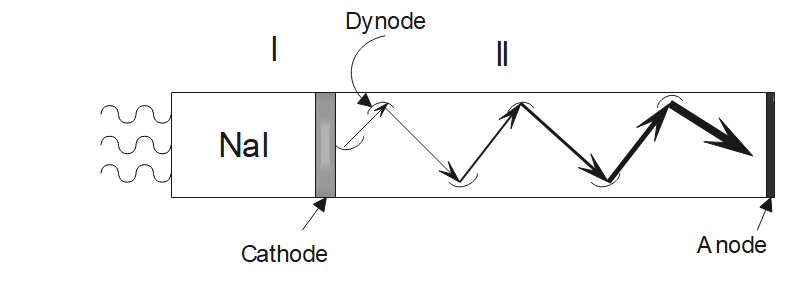
\includegraphics[scale=0.5]{ph_mult.png}	
		\caption{Φωτοπολλαπλασιαστής}
		\label{im1}
	\end{figure}			
		
\subsection*{Πειραματική Διαδικασία - Επεξεργασία Μετρήσεων}
	\subsubsection*{Βαθμονόμηση των Καναλιών}
	
		Αρχικά, όπως αναφέρθηκε θα πρέπει να βαθμονομήσουμε τα κανάλια, δηλαδή να αντιστοιχίσουμε κάθε κανάλι με μία τιμή ενέργειας.  Θα κάνουμε την αντιστοίχιση για 3 κανάλια και έπειτα θεωρώντας πως είναι γραμμική, θα την γενικεύσουμε με μία μέθοδο ελαχίστων τετραγώνων.  Γι' αυτό, θα χρησιμοποιήσουμε τρια στοιχεία των οποίων γνωρίζουμε τις ενέργειες εκπομπής ακτίνων $\gamma$. Συγκεκριμένα, θα χρησιμοποιήσουμε δείγματα $^{109}_{48}Cd$, $^{57}_{27}Co$ και $^{241}_{95}Am$. Παίρνοντας τα φάσματα βλέπουμε το κανάλι που δημιουργείται μέγιστο και αφού γνωρίζουμε την ενέργεια που του αντισοιχεί παίρνουμε τον Πίνακα (\ref{mat1}):
		\begin{table}[h!]
			\centering
			\begin{tabular}{|r|r|r|}
				\hline Ισότοπο & Ενέργεια ακτινων $\gamma$ (keV) & Channel ($\pm5$)\vspace{0.1cm} \\\hline\hline\vspace{0.1cm}
				$^{57}_{27}Co$  & 122.00  & 567 \\\hline\vspace{0.1cm}
				$^{109}_{48}Cd$ & 88.03   & 421 \\ \hline\vspace{0.1cm}
				$^{241}_{95}Am$ & 26.30   & 148 \\\hline
			\end{tabular}
			\caption{ Αντιστοιχία Καναλιών σε Ενέργεια}
			\label{mat1}
		\end{table}
		
		Από μέθοδο ελαχίστων τετραγώνων, επιβάλλοντας στην ευθεία να διέρχεται από την αρχή των αξόνων διότι θέλουμε $E(channel=0)=0keV$, προκύπτει το ότι: 
			\begin{align*}
				E_K =& A\cdot (channel) \\ 
				A   =& (0.2115	\pm 0.0054 )
			\end{align*}
			
		\begin{figure}[h!]
			\centering
			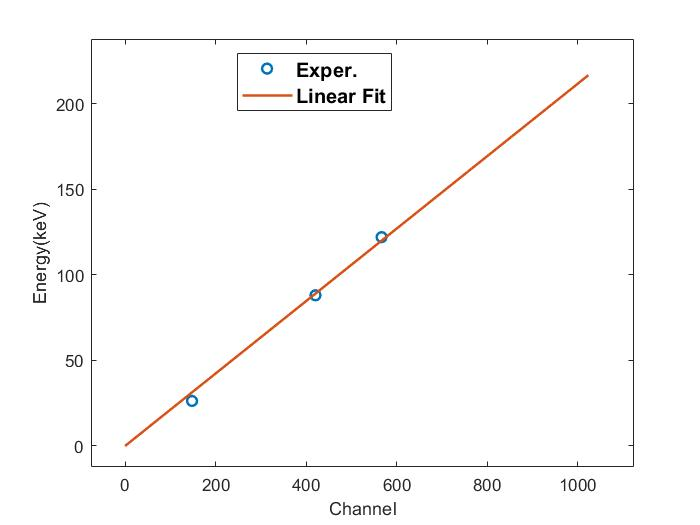
\includegraphics[scale=0.7]{channel_distr.jpg}
			\caption{Αντιστοίχιση των καναλιών σε ενέργειες}
			\label{im2}
		\end{figure}
		
%\textcolor{red}{	Για μία πρόχειρη επιβεβαίωση της αντιστοίχισής μας μπορούμε να δούμε ποιά είναι η ενέργεια της δεύτερης κορυφής των ακτίνων $\gamma$ του φάσματος του $^{241}_{95}Am$ που είναι γνωστή η θεωρητική της τιμή και είναι ίση με $59.5keV$, άρα θα έπρεπε να βρίσκεται στο κανάλι 281. Το αποτέλεσμά μας βρίσκεται στο  κανάλι .......... άρα έχει ενέργεια ....... που αποκλίνει ........... από την αναμενόμενη, άρα η βαθμονόμηση είναι ορθή.}
		
	\subsubsection*{Νόμος Moseley}
		
		Αφού έχουμε πλέον καθορίσει την ενέργεια κάθε καναλιού, μπορούμε να μετρήσουμε τις ενέργειες άγνωστων φασμάτων και κατ' επέκταση να επιβεβαιώσουμε τον ν.Moseley. Τώρα καταγράφουμε τα φάσματα εκπομπής των $^{241}_{95}Am,^{109}_{48}Cd,^{137}_{55}Cs,^{133}_{56}Ba$ και  σημειώνουμε την ενέργεια που αντιστοιχεί στο μέγιστο (η αντιστοίχηση καναλιού σε ενέργεια έχει γίνει αυτόματα από τον πρόγραμμα). Τα αποτελέσματα φαίνονται στον Πίνακα (\ref{mat2}).
		
		\begin{table}[h!]
			\centering
			\begin{tabular}{|r|r|r|r|}\hline	
				Μητρικός & Θυγρατρικός & Ενέργεια         & Αναμενόμενη  \\
				         &             & Πειραματικά(keV) & Ενέργεια(keV)\\\hline\hline
				$^{241}_{95}Am$ & $^{237}_{93}Np$ &  $100.75\pm3.00$  &  101.1 \\\hline
				$^{109}_{48}Cd$ & $^{109}_{47}Ag$ &  $18.11\pm1.00 $  &  22.2  \\\hline
				$^{137}_{55}Cs$ & $^{137}_{56}Ba$ &  $28.08\pm2.00 $  &  32.2  \\\hline
				$^{137}_{55}Cs$ & $_{82}Pb$       &  $73.12\pm2.00 $  &  75.0  \\\hline
				$^{133}_{56}Ba$ & $^{133}_{55}Cs$ &  $26.52\pm2.00 $  &  31.0  \\\hline
			\end{tabular}					
			\caption{ }
			\label{mat2}
		\end{table}
		
		Ο ν.Moseley (\ref{1}) θα ισχύει για τον θυγατρικό πυρήνα. Άρα, κάνω δυό γραφικές παραστάσεις $E_{exper.} - (Z-1)^2 $ και $E_{expected} - (Z-1)^2$. Η γραφική γίνεται με ελάχιστα τετράγωνα.
		\begin{figure}[h!]
			\centering
			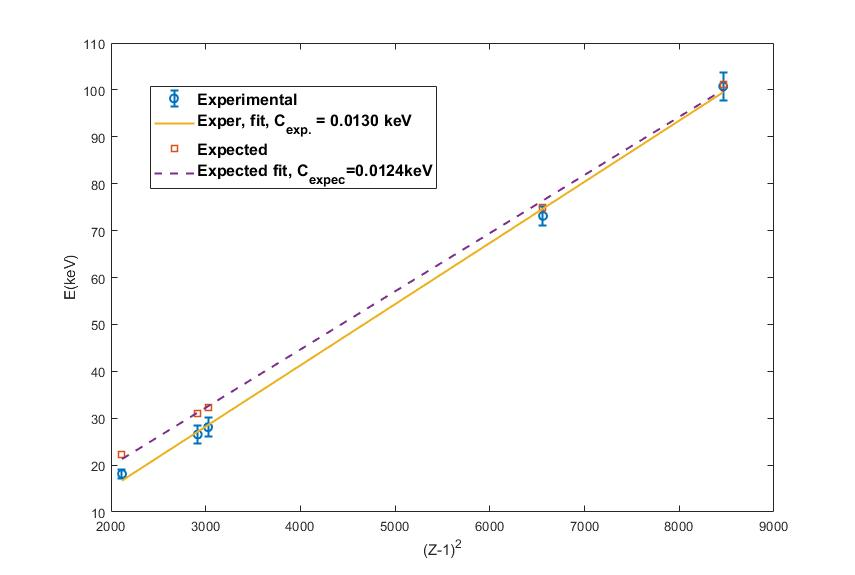
\includegraphics[scale=0.6]{moseley.jpg}
			\caption{ }
			\label{im3}
		\end{figure}
		
		Οι κλίσεις από τις μετρήσεις μας και από τα δεδομένα του Πίνακα στο φυλλάδιο προέκυψαν $C_{exp.}=(0.0130)keV$ και $C_{expect.}=0.0124keV$ αντίστοιχα. Το σχετικό σφάλμα μεταξύ πειραματικής και αποδεκτής τιμής της σταθεράς, που είναι $C=0.0102keV$, προκύπτει $\sim22\%$.
		
		
\subsection*{Συμπεράσματα}

	Εν τέλει, το αποτέλεσμα που προέκυψε αποκλίνει πολύ από την αποδεκτή τιμή, αφού το σχετικό τους σφάλμα είναι $\sim22\%$. Κάτι τέτοιο, ενδέχεται να οφείλεται στην πολυκαιρία των ραδιενεργών πηγών, οι οποίες σε αρκετά σημεία δεν έδιναν ξεκάθαρες τις κορυφές στο φάσμα (π.χ. η κορυφή των ακτίνων $\gamma$ στο $^{241}_{95}Am$). Αυτό, είχε ως αποτέλεσμα είτε την κακή βαθμονόμηση των καναλιών, είτε την λανθασμένη εύρεση της ενέργειας που αντιστοιχεί στο σωστό σημείο της κορυφής. Άρα αν είχαμε νέες πηγές, ενδεχομένως να παίρναμε καλύτερα απότελέσματα.
\end{document}